\chapter{Softwaretechnik II}

Zusammenfassung der Vorlesung "`Softwaretechnik II"' aus dem Wintersemester 2016.\footnote{\url{https://sdqweb.ipd.kit.edu/wiki/Vorlesung_Softwaretechnik_II_WS16/17}}

\section{Einführung}

\section{Gesetzmäßigkeiten}
\begin{itemize}
	\item \textit{Brook's Law}: "`Adding manpower to a late software projcet makes it later."' Gründe: Ramp-up-Time, Kommunikationsaufwand
	\item \textit{Boehm's Law}: "`Errors are more frequent during requirements and design."'
	\item \textit{Dijkstra 1969}: "`Testing shows the presence, not the absence of bugs."'
	\item (One of) \textit{Lehman's Laws}: "`A system that is used will be changed."'
	\item \textit{Parnas' Law}: "`Only what is hidden can be changed without risk"' (\(\rightarrow\) Kapselung notwendig)
\end{itemize}



\section{Software-Entwicklungsprozess}

\begin{itemize}
	\item "`Code and Fix"', als Vorgehensmodell unzureichend, da es zu schlecht strukturierten und dokumentierten Programmen führt. Darüber hinaus: Teamarbeit schwierig sowie unzureichende Skalierung
	\item Vorgehensmodell: Abstrakte Beschreibung eines Software-Entwicklungsprozesses. Beinhaltet Richtlinien bezüglich Aktivitäten, Rollen und Ergebnissen (Artefakte, Dokumente, etc.)
	\item \textbf{Wasserfallmodell}
	\begin{itemize}
		\item Phasen und Ergebnisse der Phasen
		\begin{enumerate}
			\item Planung: Lastenheft, Projektplan, Kalkulation
			\item Definition: Pflichtenheft, GUI-Beschreibung, eventuell Benutzerhandbuch
			\item Entwurf: Entwurfsdokumente, Modulführer
			\item Implementierung: Komponenten und Dokumentation, Testeinrichtung
			\item Testen: "`Fertiges"' System
			\item Einsatz und Wartung
		\end{enumerate}
		\item Probleme
		\begin{itemize}
			\item Große Softwareprojekte können i.d.R. nicht komplett (auf mehrere Jahre) geplant werden
			\item Abgrenzung der einzelnen Phasen in der Praxis oft unrealistisch
			\item Zu unflexibel bezüglich Änderungen oder Rückschritten
		\end{itemize}
	\end{itemize}
	\item \textbf{V-Modell} \\\\
	\begin{minipage}{\linewidth}
		\includegraphics[scale=0.8]{swt2/v-modell.pdf}
	\end{minipage}
	\item \textbf{Unified Process (UP)}
	\begin{itemize}
		\item Bestandteile: Entwicklungsphase, Tests, Risikomanagement
		\item Phasen
		\begin{description}
			\item[Anfangsphase:] Vergegenwärtigen des Projektumfangs, -ziels und -szenarios. Prüfen der Machbarkeit; Abschätzung des Aufwands; Kaufen vs. Entwickeln
			\item[Ausarbeitungsphase:] Entwickeln der Kernarchitektur ("`Elemente mit hohem Risiko"'); Definieren der meisten Requirements; Erstellen des Projektplans
			\item[Konstruktionsphase:] Iterative Implementierung der übrigen Elemente ("`Elemente mit niedrigem Risiko"')
			\item[Übergabephase:] Beta Tests sowie Deployment
		\end{description}
		\item Disziplinen
		\begin{description}
			\item[Business Modelling:] Erstellen eines Domänen-Modells mit Geschäftsprozessen
			\item[Requirements:] Requirements-Analyse inklusive Artefakte (Anwendungsfalldiagramme, Glossar, Vision, etc.)
			\item[Design:] Entwickeln des Umsetzungskonzepts
			\item[Implementierung, Test, Desployment]
			\item[Konfiguration, Projektmanagement]
		\end{description}
		\item Allerdings kein striktes Regelwerk vorgegeben!
	\end{itemize}
	\item \textbf{Rational Unified Process (RUP)}
	\begin{itemize}
		\item Spezifische, geregelte Umsetzung von UP. Beinhaltet Vorgaben zur Zuteilung von Aufgaben/Verantwortung innerhalb einer Organisation zur Entwicklung konkreter Produkte
		\begin{description}
			\item[Rollen (wer?):] Definiert Fähigkeiten und Verantwortlichkeiten
			\item[Aufgaben (wie?):] Beschreibt Arbeitspakete einer Rolle um Ergebnisse zu erzielen (beispielsweise Produkt)
			\item[Artefakte (was?):] Ergebnisse von Aufgaben, beispielsweise Modelle oder Dokumente 
		\end{description}
		\item Best Practices
		\begin{enumerate}
			\item Iterative Entwicklung
			\item Verwalten von Requirements
			\item Verwendung von Komponenten-basierten Architekturen
			\item Grafische Modellierung der Software
			\item Überprüfen der Software-Qualität
			\item Kontrollieren von Software-Änderungen
		\end{enumerate}
	\end{itemize}
\end{itemize}



\section{Agile Entwicklung}
\begin{itemize}
	\item Klassische Ansätze zu statisch, schwergewichtig und risikoreich
	\item \textbf{Agile Manifesto}
	\begin{itemize}
		\item Individuen und Kommunikation über Prozesse und Werkzeuge
		\item Funktionierende Software über verständliche Dokumentation
		\item Zusammenarbeit mit dem Kunden über Vertragsverhandlungen
		\item Reaktionen auf Veränderungen über das Verfolgen eines Plans
	\end{itemize}
	\item Erkenntnisse aus dem agilen Manifest: Es kann nicht jede Eventualität geplant werden; Qualität und Kundennutzen muss kontinuierlich überwacht werden
\end{itemize}

\subsection{Extreme Programming (XP)}
\begin{itemize}
	\item Sammlung aus Werten (Kommunikation, Einfachheit, Feedback, Mut) und Prinzipien (schnelle Lieferung/Feedback, Einfachheit) und Methoden
	\item \textbf{Der Prozess\footnote{\url{http://www.extremeprogramming.org/map/iteration.html}}}\\\\
		\begin{minipage}{\linewidth}
			\includegraphics[scale=0.7]{swt2/xp_iteration.pdf}
		\end{minipage}
	\item \textbf{Kritik (allgemein auch an Agile)}
	\begin{itemize}
		\item Schlechte Skalierung bei großen Projekten
		\item Fehlende Dokumentation
		\item Kunden müssen aktiv mitarbeiten
		\item Wirksamkeit mancher Methoden nicht komplett überprüft (beispielsweise Pair-Programming)
	\end{itemize}
\end{itemize}


\subsection{Scrum}
\begin{itemize}
	\item \textbf{Zusammenfassung}
	\begin{itemize}
		\item \textit{Product Owner} erstellt/verwaltet eine priorisierte Liste mit Features, dem \textit{Product Backlog}
		\item Vor jedem \textit{Sprint} entscheidet das \textit{Team} welche Features in diesem \textit{Sprint} umgesetzt werden. Diese werden in den \textit{Sprint Backlog} übernommen
		\item Das \textit{Team} koordiniert die Entwicklung im täglichen \textit{Daily Scrum Meeting}. Der Fortschritt wird in einem Burn-Down-Chart festgehalten
		\item Der \textit{Srum Master} ist für die Kommunikation im \textit{Team} verantwortlich
		\item Während jedem \textit{Sprint} wird ein (möglichst) auslieferungsbereites \textit{Product Increment} erstellt
		\item Letzteres wird vom \textit{Team} im \textit{Sprint Review Meeting} vorgestellt. Anschließend werden im \textit{Retrospective Meeting} mögliche Verbesserungen besprochen
	\end{itemize}
	\item \textbf{Sprints}
	\begin{itemize}
		\item Idealerweise konstante Dauer von höchstens einem Monat
		\item Nach jedem Sprint startet direkt der nächste \(\rightarrow\) der Entwicklungsprozess besteht aus einer Folge von Sprints
		\item Während eines Sprint dürfen keine Änderungen gemacht werden, die das Ziel gefährden oder die Quailität verringern\\\\
		\begin{minipage}{\linewidth}
			\includegraphics[scale=0.5]{swt2/scrum_process.pdf}
		\end{minipage}
	\end{itemize}
	\item \textbf{Aufgabenverteilung}
	\begin{itemize}
		\item Product Owner
		\begin{itemize}
			\item Repräsentiert den Kunden und ist für den wirtschaftlichen Erfolg des Produkts verantwortlich
			\item Erstellt/priorisiert/erklärt die Produkteigenschaften gegenüber dem Team
			\item Alleinverantwortlich für das Produkt
			\item Typische Fehler: Oft nicht verfügbar, zu wenig Durchsetzungskraft gegenüber unternehmensinternen Stakeholdern oder zu wenig technische Kenntnisse
		\end{itemize}
		\item Scrum Master
		\begin{itemize}
			\item Ist für die Umsetzung von Scrum verantwortlich
			\item Ist für die Kommunikation im Team verantwortlich
			\item Vermittelt gegenüber dem Product Owner
			\item Idealerweise ein Moderator, Coach und erfahrener Softwareentwickler
		\end{itemize}
		\item Team
		\begin{itemize}
			\item Selbstorganisierend, keine vordefinierten Rollen
			\item Idealerweise verschiedene Fachleute (GUI-Designer, Entwickler, Tester, etc.)
			\item Etwa sieben Vollzeitmitarbeiter
		\end{itemize}
		\item Kein klassischer Projektmanager vorhanden. Aufgaben werden von den drei Scrum-Rollen übernommen
	\end{itemize}
	\item \textbf{Product Backlog}
	\begin{itemize}
		\item Liste von Features, die alle Requirements beinhaltet. Nach Geschäftswert sortiert
		\item Jedes Element stellt eine User-Story da und beinhaltet eine Aufwandsangabe (\textit{Story Points})
	\end{itemize}
	\item \textbf{Sprint Backlog}
	\begin{itemize}
		\item User-Stories werden in kleinere Tasks aufgeteilt. Einzelner Task sollte nicht länger als 16 Stunden dauern
		\item Üblicherweise auf einer (non-)virtuellen Pinwand verwaltet \(\rightarrow\) bilden den Sprint Backlog
		\item Verschiedene Zustände pro Task. Beispielsweise: Todo \(\rightarrow\) In Arbeit \(\rightarrow\) Testen \(\rightarrow\) Fertig. Werden bei Zustandsänderung entsprechend verschoben/umgehängt
		\item Problem bei realen Pinwänden: Wissen geht eventuell nach Projektabschluss verloren
	\end{itemize}
	\item \textbf{Tipps für große Projekte}
	\begin{itemize}
		\item Teamgröße: Klein starten und organisch wachsen (siehe Brook's Law)
		\item Abhängigkeiten zwischen Teams verringern
		\item Daily "`Scrum of Scrums"' mit je einem (oder mehreren) Teammitgliedern
		\item Es gibt meistens einen \texttt{Sprint0}, in dem die Architektur festgelegt wird
	\end{itemize}
	\item \textbf{Tipps für verteilte Teams}
	\begin{itemize}
		\item Nach Möglichkeit vermeiden
		\item Niemals Scrum Master und Team trennen
		\item Teams erst nach Eingewöhnung trennen
	\end{itemize}
\end{itemize}


\subsection{Zusammenfassung Agile Methoden}
\begin{itemize}
	\item Vorteile: Schnelles Feedback sowie reduzierte Risiken; hatte einen großen Einfluss auf Prozessverbesserung in der Industrie
	\item Nachteile: Verwenden der selben Codebasis in verschiedenen Projekten schwierig; Skalierung unklar; hoher Anspruch an die Entwickler; Dokumentation schwierig (Projekte teilweise nur im Code dokumentiert)
	\item Tendenziell Schwächen in Architektur und Design
\end{itemize}



\section{Requirements Engineering}

\subsection{Einführung}
\begin{itemize}
	\item 48 \% aller gescheiterten Softwareprojekte scheitern an mangelhafter Anforderungsdefinition
	\item Beheben von falsch definierten Anforderungen in späteren Entwicklungsphasen kann extrem teuer sein
	\item Beschreibungskriterien: Ausreichend detailliert, komplett, widerspruchsfrei, verständlich, eindeutig, überprüfbar, risikoadjustiert
	\item Werden meist in Form von User-Stories (Agile) oder Anwendungsfällen (modellgetrieben) beschrieben
	\item \textbf{Typen von Anforderungen (concern-based Classification)}
	\begin{itemize}
		\item Funktionale Anforderungen (Functional Requirements): Verhalten der Software, beispielsweise bei der Eingabe von Daten; "`kann per Turing-Maschine beschrieben werden"'\footnote{Reussner, andere}
		\item Qualitätsanforderungen (Quality Requirements): Qualitätsmerkmale, beispielsweise Sicherheit, Bedienbarkeit, Performance
		\item Bedingungen (Constraints): Beispielsweise physikalische, rechtliche, kulturelle Umgebung oder Interface (Computerplattform)
	\end{itemize}
	\item Concern-based Kategorisierung von ANforderungen: Entsprechend dem zugrundeliegenden Anliegen ("`Concern"')
	\item Anforderungsingenieur vermittelt (als zentrale) zwischen Entwicklern und Benutzern
	\item \textbf{Anforderungsmanagementprozess}
	\begin{enumerate}
		\item Gewinnung unter Einbeziehung sämtlicher Stakeholder
		\item Dokumentation: Anforderungsspezifikation aufstellen
		\item Übereinstimmung: Finden und Aufheben von Konflikten
		\item Überprüfen und Verwalten
	\end{enumerate}
\end{itemize}


\subsection{Techniken zum Finden von Anforderungen}
\begin{itemize}
	\item Fragetechniken: Interviews, Fragebögen, On-Site-Customers
	\item Kreativtechniken: Brainstorming, Perspektivwechsel
	\item Retrospektive Techniken: Systemüberreste, Wiederverwenden, Kokurrenzsysteme
	\item Beobachtungstechniken: Feldbeobachtungen
\end{itemize}


\subsection{Grundlegende Beschreibungsempfehlungen}
\begin{itemize}
	\item Problem: Die meisten Anforderungen sind (zu Beginn) in natürlicher Sprache festgehalten
	\item Kurze Sätze, eine Anforderung pro Satz
	\item Festhalten wer für welche Aktionen/Handlungen verantwortlich ist
	\item Führen/Verwenden eines Glossars
	\item Verwenden einer Satzvorlage
\end{itemize}


\subsection{Überprüfen ob Anforderungen umgesetzt sind}
\begin{itemize}
	\item Code-Inspections, Reviews, Testfälle
	\item Simulationen, Prototyping
	\item Formale Prüfung durch \textit{Model Checking}
\end{itemize}



\section{Anwendungsfälle}

\subsection{Modelbasierte Anwenungsfallerhebung}
\begin{itemize}
	\item Anforderungsbeschreibung für Softwaresysteme durch verschiedene Modelle (textbasiert, Diagramme)
	\item \textbf{Scopes}
	\begin{description}
		\item[Business-Anwendungsfall:] Das gesamte Unternehmen (\textit{white box scope} inklusive Abteilungen und Personal)
		\item[System-Anwendungsfall:] Das gesamte Computersystem (\textit{white box scope} inklusive Komponentensicht)
		\item[Komponenten-Anwendungsfall:] Zeigt Komponenten oder Subsysteme (immer \textit{white box scope})
	\end{description}
	\item \textbf{Messen der "`Wichtigkeit"'}
	\begin{itemize}
		\item Offen unklar, wie gut/wichtig ein konkreter Anwendungsfall ist \(\rightarrow\) Fokus auf \textit{Elementary Business Processes} (EBPs)
		\item Elementary Business Process
		\begin{itemize}
			\item Definition
			\begin{itemize}
				\item Eine \textit{Aufgabe},
				\item die von einer \textit{Person} durchgeführt wird,
				\item an einem bestimmten \textit{Ort}, zu einem bestimmten \textit{Zeitpunkt},
				\item als Anwort auf ein \textit{Geschäftsereignis},
				\item die einen messbaren \textit{Geschäftswert} erzeugt und
				\item \textit{Daten} in einem konsistenten Zustand hinterlässt.
			\end{itemize}
			\item Beispiel: Prüfen einer Kreditanfrage
			\item Common Mistake: Definition zu vieler Anwendungsfälle. Besser: Formulieren von Unterandwendungsfällen
		\end{itemize}
		\item Heuristiken
		\begin{itemize}
			\item Boss-Test: Würde man dem Chef von der modellierten Tätigkeit erzählen, wenn er fragt, was man den Tag über getan hat?
			\item Kaffeepausetest: Kann der Anwender nach dem Anwendungsfall guten Gewissens eine Kaffeepause einlegen?
			\item Größentest: TODO
		\end{itemize}
	\end{itemize}
	\item \textbf{Detaillevel nach Cockburn}
	\begin{description}
		\item[1. Zusammenfassung:] Fasst mehrere Benutzerziele und Unterfunktionen zusammen
		\item[2. Benutzerziel:] Beschreibt, wie ein Benutzer eine Ziel erreichen kann
		\item[3. Unterfunktion:] "`Zwischenziel"' eines Benutzerziels
		\item[4. Zu niedrig:] Alles weitere wird als zu niedrig angesehen
	\end{description}
	\item \textbf{Anwendungsfalldiagramme}
	\begin{itemize}
		\item Textuelle Beschreibung generell wichtiger als Diagramme. Sollten nur für Zusammenfassungen/Beziehungen verwendet werden
		\item Generell auf Benutzerziel-Level 
	\end{itemize}
	\item \textbf{Finden von Anwendungsfällen}
	\begin{enumerate}
		\item Wählen der Systemgrenzen
		\item Identifizieren der primären Aktoren
		\item Identifizieren der Ziele aller Aktoren
		\item Definieren der Anwendungsfälle, um diese Ziele zu erfüllen
	\end{enumerate}
	\item \textbf{Weitere Richtlinien}
	\begin{itemize}
		\item Jeder Schritt dokumentiert einen Fortschritt im Benutzerprozess
		\item Verzicht auf UI-Details und Branches in der BEschreibung des Hauptszenarios
	\end{itemize}
\end{itemize}


\subsection{Spezifikation und Verwaltung von Anwendungsfällen}
\begin{itemize}
	\item Ziel: Vollständige Beschreibung des \textit{externen} Verhaltens einer Software \(\rightarrow\) Dokumentation aller externen Schnittstellen
	\item Zentrale Verwaltung aller Anforderungen (Datenbanken, Dokumente, Verwaltungssoftware, etc.)
\end{itemize}



\section{Verhaltensbeschreibung (Operation Contracts) und Einführung in Software-Architektur}

\subsection{Verhaltensbeschreibung (Operation Contracts)}
\begin{itemize}
	\item Formale Beschreibung des Systemverhaltens. Bestandteile:
	\begin{description}
		\item[Operation:] Name und Parameter
		\item[Cross References:] Verweise zu Anwendungsfällen, welche diese Operation beinhalten können (optional)
		\item[Preconditions:] Beschreibt Voraussetzungen zur Ausführung der Operation (beispielsweise ein bestimmter Systemzustand, siehe Geldautomat)
		\item[Postcondition:] Beschreibt mittels Domänenmodellierung den Systemzustand nach der Ausführung der Operation (im Präteritum)
	\end{description}
	\item Unterschied zu Anwendungsfällen: Contracts können einen höheren Detailgrad abdecken und werden nur bei der Notwendigkeit eines höheren Detailgrads benötigt; Contracts müssen nicht vollständig sein
\end{itemize}


\subsection{Einführung in Software-Architektur}
\begin{itemize}
	\item Architekturentwurf: Früher Zustand im Systementwurfsprozess, der Spezifikation mit Entwruf verbindet. Beinhaltet die Identifikation der wichtigesten Systemkomponenten, deren Kommunikation und deren Hardware-Ressourcen
	\item Entwurf vs. Architektur: Entwurf auf Klassenebene, Architektur auf Komponentenebene % TODO: Korrekt?
	\item Definition Software-Architektur\footnote{Reusser 2016}: Menge an Entwurfsentscheidungen, welche die Struktur eines Systems (Komponenten, Beziehungen, Deployment) beschreibt
	\item \textbf{Strutures, Views, View Points}
	\begin{itemize}
		\item Definitionen %TODO
		\begin{description}
			\item[View:] Verschiedene Sichten unterschiedlicher Stakeholder (Requirementsengineer, Architekt, SysOp, Tester) auf ein System. Beispiele: Logical/Development/Process/Physical View
			\item[Structure:] Menge der Elemente, wie sie später implementiert werden
			\item[View Point:] Zusammengefasste Sichten
		\end{description}
		\item Empfehlung: Logische Architektur und Deploymentarchitektur sollten nicht vermischt werden. Bsp.: externe Ressourcen wie Datenbanken sollten nicht als Teil der logischen Architektur dargestellt werden sondern lediglich als Teil der technischen Services ("`Persistance"')
	\end{itemize}
	\item \textbf{Vorteile einer expliziten Architektur-Dokumentation}
	\begin{itemize}
		\item Kommunikationsmedium mit expliziten Namen
		\item Vereinfachte Prüfung der nicht-funktionalen Anforderungen
		\item Wiederverwendung
		\item Projektplanung
	\end{itemize}
	\item Architektur-/Systemcharaktersistiken: Performance, Sicherheit, Verfügbarkeit, Wartbarkeit
\end{itemize}



\section{Architektur}
\begin{itemize}
	\item Neben der Architektur sollte auch der Prozess der Architekturfindung dokumentiert werden (v.a. die Motivation der einzelnen Entscheidungen)
	\item Einflussfakturen: Anforderungen, Wiederverwendbarkeit, Organisationsstruktur (zb. des Kunden), Qualitätskriterien um die nicht-funktionalen Anforderungen sicherzustellen (Performance, Skalierbarkeit, etc.)
	\item Beispiele für Architekturprinzipien: Separation of concerns (wie MVC), Single Responsibility, Information Hiding, Least Knowledge, Don't repeat yourself, Minimizing upfront design
	\item \textbf{Beispiele für Architekturstile}
	\begin{description}
		\item[Kommunikation:] Service-orientierte Architektur (SOA), Message Bus
		\item[Deployment:] Client-Server, N-Tier (zB. 3-Tier)
		\item[Struktur:] Komponenten-basiert, objektorientiert, layered (Layers \(\neq\) N-Tier)
	\end{description}
	\item Vorteile von Schichtenarchitekturen: Reduziert Komplixität; erhöht Modifizierbarkeit; Trennung der Anliegen (Concerns); vereinfacht Testen
	\item Referenzarchitektur: Generische Standardarchitektur, die als Vorlage verwendet wird
	\item \textbf{Modellierungsmöglichkeiten}
	\begin{description}
		\item[Ein Controller pro Anwendungsfall:] Gut geeignet für Systeme mit vielen Anwendungsfällen (beispielsweise \texttt{CRUD})
		\item[Einzelner (Fassaden-)Controller:] Gut geeignet für kleine Systeme mit weniger als zwölf Operationen
		\item[Direkter Objektzugang:] Reduziert Anzahl der Abstraktionsschritte mit vielen Parameterübergaben, führt allerdings zu Kontrolllogik im Domänenmodell
	\end{description}
	\item Fassaden: Ermöglichen reduzierte Schnittstellen zu Subsystemen mit vielen Klassen/Layern, die nur wenig Funktionalität exportieren
	\item Data Transfer Objects: (Serialisierte) Objekte zum Transportieren von Daten zwischen Prozessen/Komponenten etc. zur Reduzierung der Kopplung. Beinhaltet lediglich die Attribute sowie Getter und Setter (bsp. Java-Bean). Domänen-Objekte können durch ihren großen Umfang meist nicht selbst übertragen werden
	\item Domänen-Layer: Beinhaltet das Domänen-Modell und die Geschäftslogik
\end{itemize}



\section{Komponentenbasierte Software-Entwicklung}

\subsection{Einführung}
\begin{itemize}
	\item Feature-orientierte, unabhängige Einheit mit fest definierten Schnittstellen und Abhängigkeiten, die unabhängig deployt werden kann, ohne die interne Implementierung zu kennen ("`Black-Box"')
	\item Ziel: Strenge Trennung von Komponentenentwicklung und -nutzungen \(\rightarrow\) verbesserte Wiederverwendung von Komponenten
	\item Komponenten können keine Objekte sein, da Vererbung das Black-Box-Prinzip verletzt
	\item \textbf{Komponentenmodell}
	\begin{itemize}
		\item Konkrete Realisierung von komponentenbasiertem Software-Engineering
		\item Hauptproblem: Die meisten Implementierungen der letzten Jahre (\texttt{CORBA}, \texttt{EJBs}) sind eher objektorientiert als komponentenbasiert \(\rightarrow\) \texttt{OSGi}?
	\end{itemize}
\end{itemize}


\subsection{Übersicht: Technische Komponentenmodelle}
\begin{itemize}
	\item \textbf{Open Service Gateway Initiative (OSGi)}
	\begin{itemize}
		\item \textit{Bundles} als Komponentenkonzept: \texttt{JAR}-Archive mit öffentlichen Schnittstellen (per \texttt{Manifest})
		\item OSGi bietet zur Laufzeit eine Verwaltung/Registrierung der Bundles
	\end{itemize}
	\item \textbf{Web-Services}
	\begin{itemize}
		\item Selbst-beschreibende, modulare Web-Schnittstelle, die per standadrisierten \texttt{HTTP}-Aufrufen angesteuert wird
		\item Service-orientierte Architektur (SOA). Jedes Element deckt eine der folgenden Rollen ab:
		\begin{description}
			\item[Service Provider:] Publiziert Services in Service-Registrierungen
			\item[Service Requestor:] Sucht/Findet Services in Service-Registrierungen
			\item[Service Broker (Repository)] 
		\end{description}
		\item Schlüsseltechnologien
		\begin{description}
			\item[Simple Object Access Protocol (SOAP):] Spezifiziert \texttt{XML}-kodierte Nachrichten-Layouts
			\item[Web Service Description Language (WSDL):] Definiert Web-Services als Sammlung von (Netzwerk-)Endpunkten
			\item[Universal Description, Discovery and Integration (UDDI):] Ermöglicht das Finden von Web-Services durch Clients \(\rightarrow\) Basis für Repositories für Geschäftsanwendungen
		\end{description}
	\end{itemize}
	\item \textbf{Open Service Gateway Initiative (OSGi)}
	\begin{itemize}
		\item
	\end{itemize}
\end{itemize}


\subsection{Wissenschaftliche Komponentenmodelle: Palladio}
\begin{itemize}
	\item Palladio Komponenten Modell (PCM): Domänen-spezifische Modellierungssprache (DSL)\footnote{Domain specific modelling language} für Leistungsvorhersagen für Software-Architekturen in der Anfangsphase der Entwicklung
	\item Generelle Frage: Was beeinflusst die Ausführungsgeschwindig einer Komponente? - Der Algorithmus selbst, die Ablaufumgebung (beispielsweise Hardware, Virtualisierung, Betriebssystem), Performance externer Dienste, Benutzerverhalten
	\item Alle o.g. Faktoren werden im \texttt{PCM} explizit angegeben und modelliert \(\rightarrow\) ermöglicht Analysen unter verschiedenen Bedingungen (andere Ausführungsumgebung, andere Benutzung, etc.)
	\item Motivation zur Modellierung/Analyse von Software: Erweiterung von Legacy-Systemen; Leistungsvorhersagen während des Entwurfszeit (meist preiswerter als Prototypenbau); Ermittlung von Leistungsengpässen; Simulation (läuft schneller als Echtzeit); die Hardware steht eventuell noch nicht zur Verfügung (speziell bei sehr großen Software-Umgebungen)
	\item Eingabeinformationen: Komponentenmodell; Strukturmodell (inklusive externer Dienste); Deployment-Modell (Hardware, etc.); Nutzungsmodell (Datenmenge, etc.)
	\item Ausgabeinformationen: Antwortzeiten; Ressourcenauslastung; Durchsatz
	\item \textbf{Entwicklung der Modelle}
	\begin{description}
		\item[Komponenten:] Komponentenentwickler
		\item[Systementwurf:] Software-Architekt
		\item[Deployment:] System-Deployer
		\item[Nutzungsmodell:] Domänenexperte
	\end{description}
	\item \textbf{Abstrakte Verhaltensbeschreibung (SEFF\footnote{Service Effect Specification}, Aufgabenbereich des Komponentenentwicklers)}
	\begin{itemize}
		\item Ziel: Abstrakte Beschreibung des nach Außen sichtbaren Verhaltens der Komponenten \(\rightarrow\) ermöglicht die Berechnung von Laufzeiten/Ressourcenbelegung
		\item Darstellung als Aktivitätsdiagramm zur Beschreibung des Kontrollflusses
		\item Kontrollfluss wird lediglich für externe Aufruf detailliert modelliert (Abängigkeit von externen Diensten). \textit{Internal Actions} benötigen keine Modellierung des internen Kontrollflusses, da nur der Ressourcenverbrauch, nicht aber die tatsächliche Implementierung für die Laufzeitberechung relevant ist
		\item Starke Parametrisierung zur Erhöhung der Wiederverwendbarkeit der Modelle (bspw. Wahrscheinlichkeiten für Branches) \(\rightarrow\) Entkopplung von externen Einflussfaktoren. Ggf. können Parameter (wie Zugriffszeiten) erst beim Deployment festgestellt werden
		\item Aufgaben des Komponentenentwicklers
		\begin{itemize}
			\item Spezifizieren der Komponenten, Schnittstellen und Datentypen
			\item Zusammenbauen zusammengesetzter Komponenten
			\item Erstellen sowie Speichern (in Repositories) der parametrisierten \textit{SEFFs}
			\item Implementieren, testen und verwalten der Komponenten
		\end{itemize}
	\end{itemize}
	\item \textbf{Systemmodelle (Aufgabenbereich des Software-Architekten)}
	\begin{itemize}
		\item Modellieren die komponentenbasierte Architektur, die analysiert wird; inklusive exterer Komponenten und Benutzerschnittstellen
		\item Wird vom System-Deployer zum auffinden der Komponenten (in verschiedenen Repositories) benötigt
		\item Aufgaben des Software-Architekten
		\begin{itemize}
			\item Führt durch den gesamten Entwicklungsprozess
			\item Spezifiziert die Architektur (das Systemmodell) unter Verwendung \textit{existierender} Komponenten und Schnittstellen
			\item Spezifiziert \textit{neue} Komponenten und Schnittstellen
			\item Durchführung von Leistungsvorhersagen auf Basis der Architektur
			\item Überträgt Implementierungsaufgaben
		\end{itemize}
	\end{itemize}
	\item \textbf{Ressourcen (Aufgabenbereich des System-Deployers)}
	\begin{itemize}
		\item Abbildung der Komponenten auf Ressourcen
		\item Spezifiziert \textit{Resource Containers} als Laufzeitumgebung für bestimmte Komponenten inklusive abstrakter Definition der Systemressourcen (konkrete Ressourcen zum Entwurfszeitpunkt nicht bekannt). Auf Architekturebene werden in Palladio lediglich Latenz und Bandbreite angegeben
		\item Aufgaben des System-Deployers
		\begin{itemize}
			\item Modelliert die Ressourcenumgebung (Middleware, Betriebssystem, Hardware) sowie die Belegung der Ressourcen durch die Komponenten
			\item Aufbau der Ressourcenumgebung (Serverinstallation, Hardware-Konfiguration)
			\item Betreuung des laufenden Systems
		\end{itemize}
	\end{itemize}
	\item \textbf{Nutzungsmodell (Aufgabenbereich des Domänenexperten)}
	\begin{itemize}
		\item Beschreibung der Benutzung des Systems (auf der äußersten Systemschnittstelle) \(\rightarrow\) Modellierung von Verhalten (und nicht von Komponenten)
		\item Aus dem Nutzerverhalten können meist einfach Verteilungsfunktionen zu Eingaben abgeleitet werden. Palladio benötigt nur auf dieser Ebene Wahrscheinlichkeiten zur Simulation und bestimmt darauß die Verzweigungswahrscheinlichkeiten im SEFF
		\item Unterschiede zu SEFFs: Bezieht sich nicht auf Ressourcen oder innere Systemkomponenten
		\item Aufgabe des Domänenexperten: Bestimmen der Benutzeranzahl; Systemanfragen durch Benutzer sowie Charakteristiken der Eingabeparameter
	\end{itemize}
\end{itemize}



\section{Designpatterns für Enterprise Application Architecture und Microservices}
\begin{itemize}
	\item Software-Anwendungen zur Datenhaltung (CRUD) in Unternehmen
	\item \textbf{Eigenschaften von Enterprise Applications (EA)}
	\begin{itemize}
		\item Langlebige Daten: Daten bleiben länger als Anwendungen und Hardware erhalten \(\rightarrow\) oft Migration von Daten notwendig
		\item Große Datenmengen mit meist mehreren Millionen Datensätzen \(\rightarrow\) effizienter Zugriff notwendig
		\item Konkurrierender Zugriff \(\rightarrow\) Inkonsistenzen müssen verhindert werden
		\item Unterschiedliche UIs und Anwender-Typen
	\end{itemize}
	\item Vielzahl unterschiedlicher Systeme: Shops, Leasing-Management-Systeme, Ausgabenüberwachungssysteme
	\item Web Shops: Viele parallele Anwender; einfache Logic
	\item \textbf{Ebenen (Layers)}
	\begin{itemize}
		\item Präsentation: Benutzerinterface zur Informationsdarstellung und Eingabeverarbeitung
		\item Domain: Logik, Berechnungen
		\item Datenquelle: Kommunikation mit anderen Systemen, beispielsweise Datenbanken
	\end{itemize}
\end{itemize}


\subsection{Patternfamilien}
\begin{itemize}
	\item Jede Familie beschäftigt sich mit einem Problem von EAs
	\item Generell: Kein Pattern ist "`das beste"'. Wahl des Patterns aus einer Familie hängt von den konkreten Voraussetzungen ab
\end{itemize}

\subsubsection{Domain-Logik Patterns}
\begin{itemize}
	\item Mögliche Herausforderungen: Hohe Komplexität, Austauschbarkeit, Verknüpfung mit Presentation und Datenquelle(n)
	\item \textbf{Pattern: Transaction Script}
	\begin{itemize}
		\item Jede Anfrage wird in einer separaten Prozedur abgearbeitet \(\rightarrow\) sämtliche Transaktionslogik in dieser Prozedur
		\item Beispiel: Laden von Objekt aus der Datenquelle, bearbeiten des Objekts, speichern des Objekts
		\item Vorteile: Einfache, verständliche Prozeduren; unkomplizierte Verbindungen mit Datenquellen; Transaktionsgrenzen einfach feststellbar
		\item Nachteile: Skalieren schlecht bei komplexer Logik; tendenziell douplizierter Code
	\end{itemize}
	\item \textbf{Pattern: Domain Model}
	\begin{itemize}
		\item Objektmodell, das Verhalten und Datenhaltung übernimmt
		\item Objekte arbeiten für Transaction zusammen
		\item Vorteil: Bessere Organisation der Domain-Logik
		\item Nachteile: Höhere Ansprüche an Entwickler; Mapping zur Datenquelle komplexer
	\end{itemize}
	\item \textbf{Pattern: Table Module}
	\begin{itemize}
		\item Einzelne Instanz, welche die komplette Logik für eine Tabelle implementiert
		\item Entweder eine Instanz pro Datensatz oder statisch per Singleton
		\item Vorteile: Einfaches Mappen Objekt \(\leftrightarrow\) Tabellenzeile; Logiktrennung für verschiedene Konzepte; nützlich, wenn von bereits verwendeten Technologien unterstützt
		\item Nachteil: Keine Instanzen pro Objekt \(\rightarrow\) eventuell unpraktisch/nachteilig bei komplexen Anwendungen
	\end{itemize}
	\item \textbf{Entscheidungskriterien}
		\item Wichtigstes Kriterium: Komplexität der Domain-Logik
		\begin{itemize}
			\item Bei wenig Komplexität: \texttt{Table Module < Transaction Skript < Domain Model} (gemessen am Implementierungsaufwand)
			\item Bei hoher Komplexität: \texttt{Domain Model < Table Module < Transaction Skript} (gemessen am Implementierungsaufwand)
		\end{itemize}
		\item Wie aufwendig ist das Mapping zur Datenquelle?
		\item Kennen die Entwickler das Domain-Model?
		\item Welche Werkzeuge/Entwicklungsumgebungen werden verwendet?
\end{itemize}

\subsubsection{Datenquelle-Architektur-Patterns}
\begin{itemize}
	\item Ziel: Trennung von Datenbankzugriff und Domain-Logic
	\item Herausforderung: Mapping Objekt \(\leftrightarrow\) Tabellenzeile
	\item \textbf{Pattern: Record Set}
	\begin{itemize}
		\item Lokale (in-memory) Kopie von Tabellenzeile(n)
		\item Einfach zu erzeugen und zu verändern
		\item Funktionalität wird meist von Frameworks bereitgestellt und nicht selbst implementiert
	\end{itemize}
	\item \textbf{Pattern: Table Data Gateway}
	\begin{itemize}
		\item Ein Objekt als Gateway (nicht als Facade, da die Schnittstelle nicht vereinfaht wird), das den Zugriff auf alle Tabellenzeilen verwaltet
		\item Trennt Anfragen und Datenbankzugriff
		\item Implementiert \textbf{CRUD}-Methoden
		\item Geeignet für \texttt{Transaction Script}, eher ungeeignet für \texttt{Domain Model}
	\end{itemize}
	\item \textbf{Pattern: Active Record}
	\begin{itemize}
		\item Ein Objekt pro Tabellenzeile, das die Datenbankzugriff und Domain-Logic implementiert
		\item Unterschied zu \textit{Record Set}: Objekt implementiert Datenbankzugriff selbst % TODO
		\item Objektorientiert: Vereint Daten und Funktionalität
		\item Mapping muss isomorph sein
		\item Gute Wahl bei wenig komplexer Domain-Logic, ansonsten ungeeignet (bei komplexen Beziehungen oder Vererbung) \(\rightarrow\) \texttt{Data Mapper} verwenden
	\end{itemize}
	\item \textbf{Pattern: Row Data Gateway}
	\begin{itemize}
		\item Objekt, das als Gateway zu einer einzelnen Tabellenzeile fungiert. Eine Instanz pro Tabellenzeile
		\item Idee: Ähnlich wie \texttt{Active Record}, verhindert allerdings die Komplexität; kann SQL-Anfragen für verschiedene Datenbanktypen abstrahieren \(\rightarrow\) alle Zugriffsdetails sind hinter dem Interface versteckt
		\item Meist hat jede Tabelle eine Zusätzliche Finder-Klasse: \texttt{PersonFinder.find(id) \(\rightarrow\) PersonGateway}
		\item Gut geeignet für automatisch erzeugten Zugriffscode (der gesamte Datenbankzugriff wird generiert)
	\end{itemize}
	\item \textbf{Pattern: Identity Map}
	\begin{itemize}
		\item Jedes Objekt wird nur einmal aus der Datenbank geladen und dann lokal im Speicher vorgehalten (Cache)
	\end{itemize}
	\item \textbf{Pattern: Data Mapper}
	\begin{itemize}
		\item Mapping-Layer, der zwischen Datenbank und Objektspeicher vermittelt bzw. diese voneinander isoliert
		\item Mapping kann entweder explizit (für jedes Domain-Objekt existiert ein Mapper) oder Metadaten erfolgt werden, aus denen ggf. Code generiert wird
		\item Beispiel: \texttt{Hibernate}
		\item Verwendung
		\begin{itemize}
			\item Datenbankschema und Objekt-Modell entwickeln sich unabhängig (was meist der Fall ist)
			\item KomplexeBusiness-Logik, \texttt{Active Record} nicht ausreichend
			\item Automatisch erzeugt bei MDD
			\item Legacy Systeme mit bereits existierenden Datenbanken
		\end{itemize}
	\end{itemize}
\end{itemize}

\subsubsection{Sinnvolle Kombinationen aus Datenquelle-Pattern und Domain-Logic-Pattern}
\begin{itemize}
	\item \textbf{Transaction Script}
	\begin{itemize}
		\item \texttt{Row Data Gateway} oder \texttt{Table Data Gateway}
	\end{itemize}
	\item \textbf{Domain Model}
	\begin{itemize}
		\item Wenig komplexes Mapping: \texttt{Active Record}
		\item Komplexes Mapping: \texttt{Data Mapper}
	\end{itemize}
	\item \textbf{Table Module}
	\begin{itemize}
		\item \texttt{Table Data Gateway} (falls RecordSet-Framework)
	\end{itemize}
\end{itemize}

\subsubsection{Object-Relational Structural Patterns}
\begin{itemize}
	\item Mapping von OO-Strukturen zu relationalen Datenbanken (besonders bei \texttt{Domain Model} und \texttt{Data Mapper})
	\item \textbf{Pattern: Single Table Inheritance}
	\begin{itemize}
		\item Vererbungshierarchie mehrerer Klassen wird in einer einzigen Tabelle repräsentiert. Diese enthält Spalten für alle Attribute der verschiedenen Klassen sowie eine Type-Spalte
		\item Vorteile: Einfaches Datenbankschema; keine \texttt{Joins} notwendig; Verschieben von Attributen innerhalb der Hierarchie erfordert kein Anpassen der Tabelle
		\item Nachteile: Viele ungenutzte Attribute; Tabelle kann sehr groß werden; es gibt nur einen Namespace für alle Attribute (problematisch, falls mehrere Klassen gleiche Attributnamen für verschiedene Typen benutzen. Abhilfe: Naming Convention wie beispielsweise \texttt{[Classname]\_[Fieldname]})
	\end{itemize}
	\item \textbf{Pattern: Class Table Inheritance}
	\begin{itemize}
		\item Vererbungshierarchie mit je einer Tabelle pro Klasse
		\item Bei vererbten Klassen werden jeweils lediglich die neuen Attribute in der entsprechenden Tabelle gespeichert
		\item Vorteile: Einfach verständlich; Alle Spalten sind wichtig - keine Speicherverschwendung; einfaches Mapping zwischen Objekt und Datenbank
		\item Nachteile: Beim Laden eines Objekte müssen meist Daten aus mehreren Tabellen geladen werden (Leistungsverlust); aufwendigeres Refactoring; Supertypes können zum Flaschenhals werden
	\end{itemize}
	\item \textbf{Pattern: Concrete Table Inheritance}
	\begin{itemize}
		\item Jede Klasse der Vererbungshierarchie erhält eine Tabelle mit allen (auch den vererbten) Attributen
		\item Vorteile: Einfaches Zugriff, keine überflüssigen Spalten; keine \texttt{Joins} notwendig
		\item Nachteile: Verschieben von Attributen in der Hierarchie erfordert Schemaanpassung; Anpassungen bei Supertypes erfordern viele Änderungen; \texttt{find} über die Superklasse erfordert Suche in allen Subklassen (und damit Subtabellen)
	\end{itemize}
	\item \textbf{Verwendung}
	\begin{itemize}
		\item Alle Pattern in erster Linie zur Verwendung von \texttt{Domain Model} mit \texttt{Data Mapper}
		\item Abwägung zwischen Datendopplung und Geschwindigkeit
		\item Konkrete Wahl hängt von Zugriffsmustern ab
	\end{itemize}
\end{itemize}


\subsubsection{Praxis: Java Persistance API (JPA)}
\begin{itemize}
	\item Bestandteil von \texttt{Java EE}
	\item Definiert das komplette Mapping zwischen Objekt-Modell und Datenbank
	\item Kann wahlweise per \texttt{Java Annotations} oder \texttt{XML} definiert werden
	\item Vererbungspattern kann explizit festgelegt werden
\end{itemize}


\subsection{Microservices}
\begin{itemize}
	\item Architekturstil zum Entwickeln einzelner Anwendung als Sammlung kleiner, dezentraler Services
	\item Alle Services laufen als eigenständige Prozesse und kommunizieren leichtgewichtig (HTTP, RPC, etc.) \(\rightarrow\) können unabhängig mit unterschiedlichen Technologien entwickelt und deployt werden \(\rightarrow\) größere Entkopplung der Services voneinander
	\item Kann entsprechend der "`realen"' Kommunikation im Unternehmen (beispielsweise zwischen verschiedenen Abteilungen) gesehen werden
	\item "`Tolerant Reader"': Ignoriert unbekannte Anfragen \(\rightarrow\) erhöht die Robustheit
	\item Dezentrale Datenverwaltung: Jeder Service verwaltet eine eigene Datenbank
	\item Unabhängigkeit der Services eignet sich gut für automatisierte Verwaltung (beispielsweise Continuous Delivery)
\end{itemize}



\section{Software Design: Responsibility-Driven Design}

\subsection{Responsibility-Driven Design}
\begin{itemize}
	\item Zentrale Frage: Wie wird die Funktionalität auf die Objekte verteilt?
	\item \textbf{Ansätze}
	\begin{description}
		\item [Doing responsibilities:] Objekte ist für eine bestimmte Handlung verantwortlich
		\item [Knowing responsibilities:] Verantwortlichkeit auf Basis des Wissens (Objekte hält Daten)
	\end{description}
	\item \textit{Operation Contracts} als Ausgangspunkt, ggf. muss ermittelt werden, woher das verantwortliche Objekt Informationen zur Verarbeitung der Daten bekommt
	\item Verarbeitungsbeispiel: Eingabeobjekt wird an die richtige "`Bearbeitungsstelle"' weitergegeben
	\item Interaktionsdiagramme zur Ermittlung der Abläufe (wichtiger als statische Strukturdiagramme)
\end{itemize}


\subsection{Design Diagramme (Design Class Diagram)}
\begin{itemize}
	\item Interaktionsdiagramme sind eine große Hilfe beim Entwurf
	\item \textbf{Identifizieren notwendiger Klassen}
	\begin{itemize}
		\item Anforderungsliste
		\item Aus den fertigen Squenzdiagrammen können weitere Klassen abgeleitet werden
	\end{itemize}
	\item Typische Bestandteile eines Klassendiagramms: Klassen, Assoziationen, Attribute und deren Typen, Methoden, Interfaces, Abhängigkeiten
	\item Pattern \textit{Information Expert}: Verantwortlichkeit wird entsprechend vorhandenem Wissen innerhalb einer Klasse zugewiesen ("`wer die notwendigen Daten hat, ist verantwortlich"'). Existiert keine solche Klasse im Domänenmodell, muss sie ggf. hinzugefügt werden
\end{itemize}


\subsection{General Responsibility Assignment Software Patterns (GRASP)}
\begin{itemize}
	\item Systematische Beschreibung, welche Objekte für was zuständig sein sollen
	\item \textbf{Pattern: Creator}
	\begin{itemize}
		\item Legt fest, welches Objekt ein bestimmtes anderes erstellen soll (Vgl. \textit{Information Expert})
		\item \texttt{A} erstellt neues Objekt \texttt{B}, falls
		\begin{itemize}
			\item \texttt{A} eine Aggregation von \texttt{B} ist,
			\item \texttt{A} \texttt{B}-Objekte beeinhaltet,
			\item \texttt{A} \texttt{B}-Objekte mit starker Kopplung verwendet,
			\item \texttt{A} die Initialisierungsdaten für \texttt{B} hat.
		\end{itemize}
	\end{itemize}
	\item \textbf{Pattern: Controller}
	\begin{itemize}
		\item Der \texttt{Controller} oder \texttt{Facade} entscheidet über die Weiterverarbeitung von Ereignissen/Anfragen. Verstecken oft ein ganzes Subsystem
		\item Strategien
		\begin{itemize}
			\item Ein \textit{System Facade Controller}: Alle Ereignisse werden in dieser Klasse behandelt
			\item Ein Controller pro Anwendungsfall
		\end{itemize}
		\item Nicht gleichzusetzen mit einem \texttt{MVC}-Controller
	\end{itemize}
	\item Low Coupling: Niedriges Maß an Abhängigkeiten einer Klasse zu seiner Umgebung. Vereinfacht Änderungen und fördert Wiederverwendbarkeit und Verständlichkeit
	\item High Cohesion: Zusammenfassung mehrerer Komponenten, die sehr eng zusammenarbeiten
	\item Polymorphism: Verwendung von polymorphen Klassen/Methoden statt \texttt{if} für verschiedene Eingabetypen. Erhöht allerdings die Gesamtzahl an Klassen/Methoden
	\item \texttt{Kompositionen > Vererbung}. \textit{Strategie-Pattern}: Verhalten wird zur Laufzeit konfiguriert. Vereinfacht die Entwicklung, da zur Vererbung die Implementierung der Oberklasse bekannt sein muss (Blackboxtechnik vs. Whiteboxtechnik). Erhöht die Flexibilität (siehe Entenbeispiel)
	\item Pure Fabrication: Wird verwendet, um einen Algorithmus zu kapseln, der in keine Domain-Klasse passt. Beispielsweise um Technologiewissen von Domänenwissen zu trennen. Sie implementiert reines Verhalten und hat somit keinen Zustand. Sollte nicht zu häufig verwendet werden, sonst existieren am Schluss nur noch Klassen die einzelne Methoden kapseln.\footnote{\url{https://de.wikipedia.org/wiki/GRASP\#Pure_Fabrication}}
	\item Indirection: Indirection (Umweg) kann verwendet werden um geringe Kopplung zu erreichen (Weitergabe von Verantwortlichkeit). Sie wird erreicht, indem ein Vermittler zwischen Client und Server eingebaut wird. Sinnvoll wenn sich ein Serverobjekt ständig verändert. Als Nachteil ist die Leistungsfähigkeit vermindert. Beispielhaft für dieses Muster ist die Einführung der Controller-Komponente, die zwischen dem Datenmodell (Model) und dessen Präsentation (View) im Model-View-Controller-Architekturmuster vermittelt.\footnote{\url{https://de.wikipedia.org/wiki/GRASP\#Indirection}}
	\item Protected Variations: Interfaces sollen immer verschiedene konkrete Implementierung verstecken. Man nutzt also Polymorphismus und Delegation, um zwischen den Implementierungen zu wechseln. Dadurch kann das restliche System vor den Auswirkungen eines Wechsels der Implementierung geschützt werden.\footnote{\url{https://de.wikipedia.org/wiki/GRASP\#Protected_Variations}}
\end{itemize}



\section{Modellgetriebene Entwicklung (Model Driven Development)}

\subsection{Motivation und Einführung}
\begin{itemize}
	\item "`Metamodell"': Modell um Modelle zu beschreiben
	\item Ziele von MDD: Plattformunabhängigkeit; höhere Entwicklungsgeschwindigkeit; bessere Softwarequalität; Wiederverwendbarkeit
	\item Erwartete Vorteile: Kostenreduzierung; kürzere Time-to-Market; variabel
\end{itemize}


\subsection{Modellgetriebene Software-Entwicklung}
\begin{itemize}
	\item \textit{Domain Expert} künftig für die Entwicklung von Anwendersoftware verantwortlich
	\item Modelle reduzieren die Komplexität, sind (automatisch) analysierbar, verbesseren die Kommunikationseffizienz
	\item \textit{Model-Driven}: Modelle sind primäre Artefakte, anstelle des Sourcecodes und damit unverzichtbarer Teil des Entwicklungsprozesses
	\item \textit{Model-Based}: Modelle sind sekundäre Artefakte, die beispielsweise für die Dokumentation erstellt werden
\end{itemize}

\subsection{Model Driven Architecture (MDA)}
\begin{itemize}
	\item MDD-Implementierung
	\item Bietet Standardisierung
	\item Verwendet existierende Standards
	\item \textbf{Modellformen}
	\begin{itemize}
		\item Computing Independent Models (CIM)
		\begin{itemize}
			\item Umgangssprachliche Beschreibung
			\item Klassendiagramm mit Klassenattributen aber ohne Klassenmethoden
		\end{itemize}
		\item Platform Independent Models (PIM)
		\begin{itemize}
			\item Plattformunabhängiges Modell für Geschäftsprozesse
			\item Hinzufügen von Methoden (und eventuell zusätzlichen, technischen Attributen) zum Klassendiagramm
		\end{itemize}
		\item Platform Specific Models (PSM)
		\begin{itemize}
			\item Plattformabhängiges Modell für Architektur/Services
			\item Ersetzen von generischen Typen durch plattformspezifische
		\end{itemize}
		\item Transformationen (Abstrakte Ebene \(\rightarrow\) Code-Ebene)\\\\
		\begin{tikzpicture}
			\node at (0, 0) [rectangle,draw] (cim)  {\(CIM\)};
			\node at (3, 0) [rectangle,draw] (pim)  {\(PIM\)};
			\node at (6, 0) [rectangle,draw] (psm)  {\(PSM\)};
			\node at (9, 0) [rectangle,draw] (code) {\(Code\)};

			\draw[->] (cim) edge node {} (pim);
			\draw[->] (pim) edge node {} (psm);
			\draw[->] (psm) edge node {} (code);
			\draw[<-] ($(pim.east)!0.5!(psm.west)$) -- ++(0,1cm) node[above] {Plattformmodell}; 
		\end{tikzpicture}
	\end{itemize}
\end{itemize}


\subsection{Schlüsselkonzepte und Definitionen}

\subsubsection{Metamodeling}
\begin{itemize}
	\item Vereinfachtes UML-Klassendiagramm
	\item Müssen immer vollständig sein, d.h. bereits alle Attribute/Typen und Assoziationen/Aggregationen enthalten, da sie automatisch weiterverarbeitet werden
\end{itemize}

\subsubsection{Model Transformation}
\begin{itemize}
	\item Transformation: \texttt{Meta-Model\_A} \(\longrightarrow\) \texttt{Meta-Model\_B} nach vorgegebenen Regeln
\end{itemize}


\subsection{Sprachen und Werkzeuge}
\begin{itemize}
	\item \textbf{Eclipse Modeling Framework (EMF)}
	\begin{itemize}
		\item De-facto MDD-Standard
		\item Wird von vielen großen Firmen und Projekten verwendet
	\end{itemize}
	\item \textbf{Essential Meta-Object Facility (EMOF)}
	\begin{itemize}
		\item Von der \textit{Object Management Group} (OMG) als Metadaten-Architektur definiert
	\end{itemize}
\end{itemize}

% TODO Rest ab Folie #48


\subsection{Forschung und Praxis}



\section{Clean Code}
\begin{itemize}
	\item \textbf{Motivation}
	\begin{itemize}
		\item Schlechter Code senkt die Produktivität exponentiell
		\item Lesbarkeit extrem wichtig, da Code i.d.R. öfters gelesen als geschrieben wird
		\item Guter Code erhöht die Wartbarkeit ("`a system that is used will be changed"'\footnote{Lehman's first law} sowie "`an evolving system increases its complexity unless work is done to reduce it"'\footnote{Lehman's second law})
		\item Verwendung iterativer/inkrementeller Methoden (Agile) erreicht durch Refactern, dass die Komplexitätskurve flach bleibt
	\end{itemize}
\end{itemize}


\subsection{Die fünf SOLID-Prinzipien für gutes OO-Design}
\begin{enumerate}
	\item \textbf{Single Responsibility Principle (SRP)}
	\begin{itemize}
		\item Klassen sollen lediglich eine einzige Verantwortlichkeit haben (Definition "`Anzahl Verantwortung"' über die Anzahl der Änderungsgründe)
		\item Ggf. müssen Klassen aufgeteilt werden (Bsp. Modem: Funktionalität nach Verbindungsverwaltung und -nutzung aufteilen)
		\item Verbessert die Lesbarkeit und verringert das Fehlerrisiko
		\item Command-Query-Separation: Trennung von Methoden, die manipulieren/zurückliefern (verringert Seiteneffekte, einfacher testbar, Queries sollten immer das selbe Ergebnis liefern, vgl. Idempotenzgesetz). Ausnahme: Iterator
	\end{itemize}
	\item \textbf{Open Closed Principle (OCP)}
	\begin{itemize}
		\item Softwareeinheiten sollen unkompliziert erweitert, aber nicht verändert werden können: "`Verändern durch Ergänzen"'
		\item Beispiel: Zeichnen verschiedener Grafikprimitive durch Vererbung statt \texttt{Switch} (Methodenverschiebung nach Unterklasse)
	\end{itemize}
	\item \textbf{Liskov Substitution Principle (LSP)}
	\begin{itemize}
		\item Unterklassen müssen immer in Oberklassen einsetzbar sein
		\item Das Ersetzbarkeitsprinzip fordert, dass eine Instanz einer abgeleiteten Klasse sich so verhalten muss, dass jemand, der meint, ein Objekt der Basisklasse vor sich zu haben, nicht durch unerwartetes Verhalten überrascht wird, wenn es sich dabei tatsächlich um ein Objekt eines Subtyps handelt\footnote{\url{https://de.wikipedia.org/wiki/Prinzipien_objektorientierten_Designs\#Liskovsches_Substitutionsprinzip}}
		\item Verletzung des Prinzips häufig nicht auf den ersten Blick erkennbar
		\item Beispiel: \textit{Quadrat} darf nicht von \textit{Rechteck} erben, da durch \texttt{setHeight()} oder \texttt{setWidth()} der Oberklasse, \textit{Quadrate} regelwidrig geändert werden könnten (allgemein: Vererbung unpassender/sinnloser Methoden)
	\end{itemize}
	\item \textbf{Interface Segregation Principle (ISP)}
	\begin{itemize}
		\item Dient dazu, große Interfaces aufzuteilen
		\item Die Aufteilung soll gemäß der Anforderungen der Clients an die Interfaces gemacht werden - und zwar derart, dass die neuen Interfaces genau auf die Anforderungen der einzelnen Clients passen. Die Clients müssen also nur mit Interfaces agieren, die das, und nur das können, was die Clients benötigen\footnote{\url{https://de.wikipedia.org/wiki/Prinzipien_objektorientierten_Designs\#Interface-Segregation-Prinzip}}
		\item Beispiel: Industrieroboter vs. Mensch. Ein Mensch benötigt mehr Zugriffe (essen, trinken,...)
	\end{itemize}
	\item \textbf{Dependency Inversion Principle (DIP)}
	\begin{itemize}
		\item Abhängigkeiten sollten immer von konkreteren Modulen niedriger Ebenen zu abstrakten Modulen höherer Ebenen gerichtet sein\footnote{\url{https://de.wikipedia.org/wiki/Prinzipien_objektorientierten_Designs\#Dependency-Inversion-Prinzip}}
		\item Verwendung von Interfaces statt direkter Implementierung \(\rightarrow\) Invertierung der Abhängigkeit 
	\end{itemize}
\end{enumerate}


\subsection{Weitere Prinzipien}
\begin{itemize}
	\item \textit{Law of Demeter}: Objekte sollen nur mit Objekten in ihrer unmittelbaren Umgebung kommunizieren. Dadurch soll die Kopplung in einem Softwaresystem verringert und dadurch die Wartbarkeit erhöht werden\footnote{\url{https://de.wikipedia.org/wiki/Prinzipien_objektorientierten_Designs\#Gesetz_von_Demeter}}
	\item \textit{Boy Scout Rule}: Code wird mit der Zeit schlechter \(\rightarrow\) regelmäßiges Refactern (beispielsweise vor dem Commiten)
	\item \textit{Principle of least Surprise}: Funktionen und Klassen sollten implementieren, was von ihnen erwartet wird (Intuitivität). Typische Abkürzungen oder Großundkleinschreibung sollten akzeptiert werden
	\item \textbf{Code Conventions}
	\begin{itemize}
		\item Namen sollten präzise sein (\texttt{getThem()} vs. \texttt{getFlaggedCells()})
		\item Naming: Innerhalb eines Projekts/Teams standardisiert; aussagekräftig; Vermeidung unnötiger Pre-/Postfixes
		\item Commenting: Aussagekräftig; Verschieben von komplexen Kontrollstrukturen (die aufwendig kommentiert werden müssen) in Methoden
	\end{itemize}
	\item \textit{Don't repeat yourself} (DRY): Führt zu Fehlern und Inkonsistenzen. Vermindert Wartbarkeit, Verständlichkeit, Erweiterbarkeit
	\item \textit{Keep it simple (KISS)}: Erhöht die Verständlich. Beispiel: Verzicht auf unnötig komplexe Datenstrukturen
	\item \textit{You ain't gonna need it} (YAGNI): Features sind teuer/aufwendig (mehr Testing/Dokumentation). Implementiere lediglich was nötig ist
	\item \textit{Single Level of Abstraction} (SLA): Statements innerhalb einer Funktion/Funtionen innerhalb einer Klasse sollten auf dem selben Abstraktionslevel sein
\end{itemize}


\subsection{Clean Architecture}
\begin{itemize}
	\item Verschiedene Architekturmuster: Hexagonale Architektur; Zwiebelarchitektur \(\rightarrow\) gemeinsames Ziel: Verwendung von Layern
	\item Ziele: Unabhängige Frameworks; gute Testbarkeit; Unabhängigkeit von UI, Datenbank und externe Abhängigkeiten
	\item Abhängigkeiten existieren nur von Außen nach Innen ("`The Dependency Rule"')
	\item \textbf{Schichtenmodell (von Innen nach Außen)}
	\begin{description}
		\item[Entities:] Anwendungsunabhängige Daten inklusive elementarer Operationen auf diesen Daten ohne komplexe Logik
		\item[Use Cases:] Anwendungsabhängige Daten in Domänenterminologie. Keine Abhängigkeit zu UI oder konkreter Datenbankrealisierung (beides ebenfalls nicht in der Anwendungsfallbeschreibung enthalten)
		\item[Interface Adapters:] Kommunikation mit externen Diensten (UI, Datenkonversion)
	\end{description}
\end{itemize}


\subsection{Refactoring}
\begin{itemize}
	\item Definition: Änderungen am Source-Code, die das Verhalten des Programms nicht beeinflussen
	\item Methoden wachsen während der Entwicklung dynamisch \(\rightarrow\) müssen ggf. aufgesplittet werden
	\item Grundlage zur Code-Qualität: Testcases
	\item Anwendungsbeispiele, die Refactoring notwendig machen: Lange Methoden; doppelter Code; (zu) große Klassen, etc.
\end{itemize}



\section{Design Patterns für Echtzeitsysteme}

\subsection{Grundlagen}
\begin{itemize}
	\item Echtzeitanforderung: System \textit{muss} innerhalb einer vorgegebenen Zeit antworten
	\item "`Harte Echtzeitanforderung"': Daten sind korrekt, wenn sie zeitlich und logisch korrekt sind
	\item "`Weiche Echtzeitanforderung"': Antwortzeit muss innerhalb einer Toleranz liegen (beispielsweise Mittelwert als Kriterium). Die vorgegebene Antwortzeit kann regelmäßig überschritten werden
	\item Typische Anwendungen: Monitoring, Kontrollsysteme, Data Acquisition Systems
	\item Sensor-Aktor-Schema (wird meist als Schleife ausgeführt)\\\\
		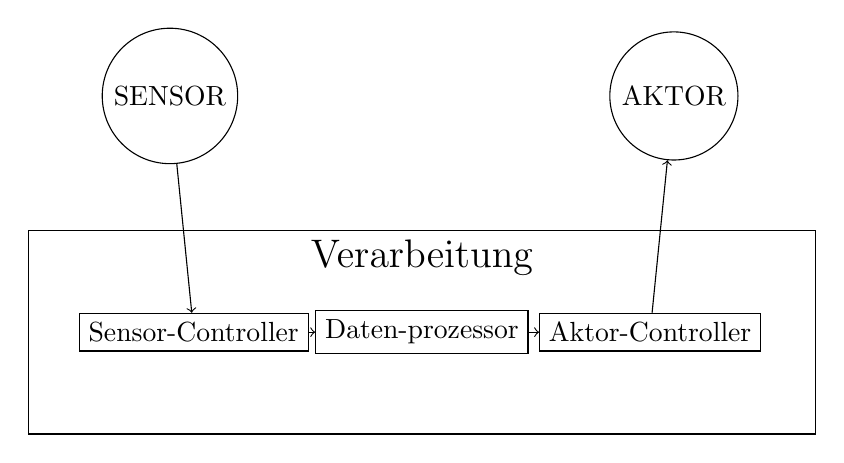
\begin{tikzpicture}
			\node at (-3.2, 3) [circle,draw] (sensor) {SENSOR};
			\node at ( 3.2, 3) [circle,draw] (actor)  {AKTOR};
			\node at (   0, 0) [rectangle,draw,text depth = 2cm,minimum width=10cm,font=\Large] (processing){Verarbeitung};

			\node at ([xshift=6em]processing.west)  [rectangle,draw] (sensor_controller) {Sensor-\\Controller};
			\node at (processing.center)            [rectangle,draw] (data_processor)    {Daten-\\prozessor};
			\node at ([xshift=-6em]processing.east) [rectangle,draw] (sensor_actor)      {Aktor-\\Controller};

			\draw[->] (sensor)            edge node {} (sensor_controller);
			\draw[->] (sensor_controller) edge node {} (data_processor);
			\draw[->] (data_processor)    edge node {} (sensor_actor);
			\draw[->] (sensor_actor)      edge node {} (actor);
		\end{tikzpicture}
	\item Herausforderungen: Viele verschiedene Sensoren mit unterschiedlichen Echtzeitbedingungen
\end{itemize}


\subsection{Echtzeitbetriebssysteme}
\begin{itemize}
	\item "`Normale"' Betriebssysteme ungeeignet, da sie viel unnötigen Overhead (Dateimanagement, Netzwerk, UI, etc) \(\rightarrow\) Echtzeitbetriebssysteme auf Echtzeitanwendungen spezialisiert
	\item \textbf{Bestandteile}
	\begin{itemize}
		\item Echtzeitsystemuhr (\textit{real-time clock})
		\item \textit{Interrupt Handler}
		\item \textit{Scheduler}: Bestimmt, welcher Prozess als nächstes ausgeführt wird
		\item \textit{Resource Manager} zum Verwalten von Speicher-/Prozessresourcen
		\item \textit{Dispatcher} zum Ausführen von Befehlen/Anwendungen (nachdem der Scheduler einen Prozess ausgewählt hat)
	\end{itemize}
	\item \textbf{Prioritätslevel}
	\begin{description}
		\item[Interrupt-Level:] Höhere Priorität für unregelmäßig auftretende Prozesse, die eine schnellere Antwort erwarten
		\item[Clock-Level:] Periodische Prozesse
	\end{description}
	\item \textbf{Scheduling}
	\begin{itemize}
		\item Bestandteile
		\begin{description}
			\item[Scheduler:] Wählt den nächsten Prozess, der vom OS ausgeführt wird
			\item[Resource Manager:] Allokiert Systemressourcen (Prozessor, Speicher, etc.)
			\item[Dispatcher:] Für die eigentliche Prozessausführung verantwortlich
		\end{description}
		\item Statisch (Gesamtanzahl der Prozesse im System unveränderlich) oder dynamisch
		\item Scheduling-Strategien
		\begin{itemize}
			\item \texttt{First-In-First-Out (FIFO)}: dynamisch, non-preemtive, keine Prioritäten
			\item \texttt{Fixed-Priorities}: Entsprechend dynamischen oder statischen Prioritäten
			\item \texttt{Earliest-Deadline-First (EDF)}: dynamisch, dynamische Prioritäten
			\item \texttt{Least-Laxity-First (LLF)}: \(laxity = deadline-now-t_{remaining\_processing\_time}\). Kein Kontextwechsel bei gleicher Laxity zweier Prozesse
			\item \texttt{Time-Slice-Scheduling}: Iterativ mit Warteschlange und unterschiedlich langen Time-Slices pro Prozess. Neue Prozesse werden beim Eintreffen hinten die Warteschlange eingefügt
		\end{itemize}
	\end{itemize}
	\item \textbf{Java zur Entwicklung echtzeitfähiger Anwendungen}
	\begin{itemize}
		\item Klassisch: JVM ungeeignet für Echtzeitanwendungen (Garbagecollector sowie JustInTime-Compilation nicht drterministisch)
		\item Vorteile von Java gegenüber C/C++ allerdings auch in Echtzeitanwendungen gewünscht (besser umgesetzte OO, portabler, bessere Hardwarabstraktion, etc.)
		\item \texttt{JamaicaVM}\footnote{Realtime-Java aus Karlsruhe}: Anpassungen der JVM zur Unterstützung von Echtzeitanwendungen sowie angepasste Programmierung notwendig (deterministische Ausführung von Schleifen, etc.)
	\end{itemize}
\end{itemize}


\subsection{System Design}
\begin{itemize}
	\item Ausgangsfrage: Welche Teile werden in Hardware (schneller und teurer), welche Teile werden in Software umgesetzt? \(\rightarrow\) Entscheidung auf Basis der Qualitätskriterien
	\item \textbf{RT-Entwurfsprozess}
	\begin{enumerate}
		\item Identifizierung von Stimuli und Antworten
		\item Bestimmen der Zeitbedingungen
		\item Festlegen der Ausführungsplattform (Hardware, RTOS, etc.)
		\item Definition der parallel ablaufenden Prozesse (ergibt sich aus Gruppierung von (1))
		\item Implementierung der Antworten (Modellierung mittels Zustandsautomaten: Ausgabe abhängig von Eingabe und Zustand)
		\item Entwurf des Schedulings
	\end{enumerate}
	\item \textbf{Thread-Kommunikation}
	\begin{description}
		\item[Shared-Memory:] Kommunikation über gemeinsamen Speicher
		\item [Message-Passing:] Kommunikation über (non-)blocking, (a-)sychrone Weitergabe von Nachrichten
	\end{description}
	\item \textbf{Safety vs. Reliability} % TODO
	\begin{description}
		\item[Safety:] System kann ohne zuverlässig betrieben werden
		\item[Reliability:] Wahrscheinlichkeit, dass ein System fehlerfrei arbeitet
	\end{description}
\end{itemize}


\subsection{Echtzeit-Muster}
\begin{itemize}
	\item \textbf{Channel (oder auch Pipe/Filter)}
	\begin{itemize}
		\item Fließbandartige Verarbeitung der Daten mit vielen Zwischenstationen, die jeweils eine abgeschlossene, triviale Operation übernehmen
		\item Verbesserung: Verwendung mehrerer Channels für höhere Leistung und Zuverlässigkeit
	\end{itemize}
\end{itemize}



\section{Zuverlässigkeit und statistisches Testen}
\begin{itemize}
	\item Wie viel Testen ist genug? - Abbruchkriterien: Zeit/Budget ausgebraucht; Zielgröße bei Code-Coverage erreicht; alle Testfälle Funktionierende
	\item Definition "`Zuverlässigkeit"': Wahrscheinlichkeit, dass ein System fehlerfrei arbeitet
	\item \textbf{Ansätze}
	\begin{description}
		\item[Functional Testing:] Testen der Benutzerfunktionen
		\item[Coverage Testing:] Testen sämtlicher Code-Pfade
		\item[Random Testing:] Testen zufällig generierte Eingabedaten
		\item[Partition Testing:] Testdaten werden zufällig aus verschiedenen Bereichen ausgewählt und getestet
		\item[Statistical Testing:] Nutzung experimentell ergeugter Eingabedaten
	\end{description}
	\item Generelles Problem: Nur ein kleiner Teil der möglichen Eingabedaten kann getestet werden. Wie wird diese Teilmenge ausgewählt?
	\item \textbf{Statistisches Testen}
	\begin{itemize}
		\item Voraussetzung: Nutzungsmodell der Software; Simulation der Betriebsumgebung; Protokoll zur Analyse der Testdaten \(\rightarrow\) das Modell erzeugt statistisch korrekte Testdaten für alle Anwendungsmöglichkeiten
	\end{itemize}
	% TODO: Formeln
	\item \textbf{Nutzungsbasiertes statistisches Testen}
	\begin{itemize}
		\item Voraussetzungen
		\begin{enumerate}
			\item Es existiert ein verlässliches Nuzungsprofil (Beispiel auf Basis eines Markov-Modells \(\rightarrow\) Berechnung aller Code-Pfade; Berechnung zufälliger Code-Pfade mittels Random-Walk)
			\item Die Testfälle sind statistisch unabhängig von (vorherigen) Tests (Software muss zwischen Testläufen immer in den Orginalzustand zurückgesetzt werden, sonst entstehen kaskadierende Zustandsänderungen)
			\item Erkennen, ob ein Test erfolgreich war oder nicht
		\end{enumerate}
	\end{itemize}
	\item \textbf{Weitere Vorteile bei Verwendung eines Benutzungsmodells}
	\begin{itemize}
		\item Entstehung im Rahmen der Anforderungserhebung
		\item Wahrscheinlichere Pfade können öfters/besser getestet werden
		\item Partitionierung der Concerns
		\item Entdecken von Optimierungsmöglichkeiten (beispielsweise im UI)
	\end{itemize}
\end{itemize}



\section{Einführung in Software-Sicherheit}
\begin{itemize}
	\item Motivation: Unsichere Software ist teuer (Downtime; hohe Kosten beim Schließen von Sicherheitslücken)
	\item \textbf{Gründe für unsichere Software}
	\begin{itemize}
		\item Kein Geld oder keine Zeit zum Testen
		\item Schlechtes Design
		\item Implementierungsfehler
	\end{itemize}
	\item Optimal: Sicherheitsanforderungen bereits im Entwurf integrieren ("`Security by Design"')
	\item \textbf{Sicherheitsanforderungen}
	\begin{itemize}
		\item Präzise Beschreibung der Schutzanforderungen: Vor wem? wieso? wie lange?
		\item Schlecht: "`Use encryption wherever necessary"'
		\item Besser: "`Protect credit card data from unauthorized access because this information is sensitive"'
		\item Wichtig: Annahmen bei Entwurfsentscheidungen dokumentieren (Beispiel: Feldbus im Auto nur unter der Motorhaube zugreifbar)
	\end{itemize}
	\item \textbf{Grundprinzipien für sichere Software}
	\begin{enumerate}
		\item "`Schwächste"' Angriffslinie schützen
		\item Mehrere kaskadierende Sicherheitsmaßnahmen, falls eine davon durchbrochen wird
		\item Sichere Ausnahmebehandlung (beipsielsweise keine Stacktraces anzeigen)
		\item Sicherheitseinstellungen initial so hoch wie möglich. Benutzer muss Ausnahmen etc. selbst hinzufügen
		\item Principle of least privilege
		\item No security by obscurity\footnote{Kerkhoffs Prinzip}
		\item Angriffsfläche minimieren (weniger Code bietet weniger Angriffsfläche; welche APIs werden exportiert; etc.)
		\item Software-Kern mit hohen Berechtigungen speziell schützen (beispielsweise durch formale Verifikation)
		\item Prüfen der Eingabedaten. Eingabedaten dürfen nicht als Code verwendbar sein (SQL-Injection, etc.)
		\item Trennen von Code und Daten (kein hartkodiertes Kennwort)
	\end{enumerate}
	\item \textbf{Weitere hilfreiche Muster}
	\begin{enumerate}
		\item Verwendung existierender Systeme zur föderativen Benutzerverwaltung (LDAP, etc.)
		\item Sinnvolle Passwörter (beispielsweise lange Passphrases statt Regeln zu Sonderzeichen); Passwörter nicht client-seitig validieren (Client-Seite generell unsicherer); salten; padden
		\item Verschlüsselte Verbindungen bei Session-Handling
	\end{enumerate}
	\item \textbf{Implementierung}
	\begin{itemize}
		\item Die meisten Sicherheitslücken entstehen durch Implementierungsfehler (Bufferoverflow in \texttt{C})
		\item Sicherheitsrichtlinien
		\begin{enumerate}
			\item Sicherheitstest sind nicht das gleiche wie Funktionstests. Ziel: Finden von Schwachstellen
			\item Selten genutzten Code ebenfalls ausführlich testen (Auffinden durch Coverage-Analyse). Ungenutzter Code ist oft der gefährlichster
			\item Reviews durch Sicherheitsprofis
			\item Verwendung einer Sicherheitstestumgebung (Port-Scans, Intrusion Detections, etc.)
			\item Blackbox- und Whitebox-Tests durch spezialisierte Firmen
			\item 
		\end{enumerate}
		\item Sicherheitszertifizierungen
		\item Angriffsbeispiele
		\begin{itemize}
			\item Race Conditions
			\begin{itemize}
				\item Beispiel: Test der Zugriffsberechtigung auf eine Datei, bevor sie geöffnet wird. Prüfung und Öffnung erfolgt via Dateinamen
				\item Problem: Umbiegen des Dateinamens auf eine andere Datei, zwischen Prüfen und Öffnen (in einer nebenläufigen Umgebung möglich)
				\item Gegenmaßnahmen: Verwendung von Dateipointern oder Critical Sections
			\end{itemize}
			\item Buffer Overflows
			\begin{itemize}
				\item Manche \texttt{C/C++}-Befehle prüfen beim Anlegen eines Buffers keine Speichergrenzen \(\rightarrow\) Zugriff auf Daten oder Code eines anderen Speicherbereichs möglich
				\item Beispiel: \texttt{char buf[BUFSIZE]; gets(buf);}. Platziert Schadcode in einer anderen Anwendung
				\item Besser: Ersetzen durch \texttt{char buf[BUFSIZE]; fgets(buf, BUFSIZE, stdin);} (liest nur bis zum Zeilenumbruch)
			\end{itemize}
			\item SQL-Injection
			\begin{itemize}
				\item Ziel: Erweitern des SQL-Befehls durch Hinzufügen an String-Eingabe
				\item Lösung: PreparedStatements; Prüfen der Eingabe
			\end{itemize}
		\end{itemize}
	\end{itemize}
\end{itemize}



\section{Continuous Integration}
\begin{itemize}
	\item Ziel: Sicherstellen der Qualität durch funktionale und qualitative Tests in einer repräsentativen Umgebung; Erhöhung der Transparenz
	\item Integration in den Release-Prozess: Bei jeder Änderung werden automatisierte Tests durchgeführt und ein Release erzeugt (\textit{Continuous Delivery})
	\item \textbf{Voraussetzungen}
	\begin{itemize}
		\item Verwendung automatisierter Software-Builds (Ant, Maven, make, etc.)
		\item Unittests und Integrationtests
		\item Testing-Automation
	\end{itemize}
	\item \textbf{Best-Practices}
	\begin{itemize}
		\item Verwendung eines zentralen Entwicklungs-Repsitory für alle Entwicklungsartefakte (Quell-Code, Tests, Scripte, etc.)
		\item Vermeidung duplizierten Test-Codebasis
		\item \textit{Design for fast Feedback}: Kritische Tests zuerst; Unittests vor Integrationtests
		\item Ein Build-System für jegliche Verwendung (lokaler Test; Integrationbuild; Release)
		\item Automatisierte Zusammenfassung der Fehler an den Verursacher
		\item Gute Komponentisierung für Komponenten-basiertes Testen
	\end{itemize}
	\item Continuous Delivery: Erweiterung zu CI; Builds werden nach zusätzlichem Akzeptanztest durch das Test-Team direkt freigegeben
	\item Ergebnis einer Studie zur Code-Qualität von CI-unterstützten Projekte auf Github: Effektivere Zusammenarbeit durch einfachere Integration von (zuvor getesteter) Pull-Requests; Code-Qualität insgesamt durch mehr gefundende Bugs verbessert
\end{itemize}



\section{Reviews}
\begin{itemize}
	\item \textbf{Terminologie}
	\begin{description}
		\item[Validierung:] Fallbasiertes Testen
		\item[Verifizierung:] Formale Betriebsprüfung. Bei erhöhter Komplexität i.d.R. nicht durchführbar (zu viele Pfade zum Testen; Annahmen zur Gleitkommaaritmetik oder Speicherbelegung)
		\item[Review:] Menschen untersuchen Artefakte auf Korrektheit
	\end{description}
	\item Können bereits in frühen Phasen eingesetzt werden, wenn Werkzeuge noch nicht zur Verfügung stehen
	\item Motivation: Früh gefundene Fehler sind generell einfacher/günstiger zu beseitigen
	\item \textbf{Wieso nicht häufiger eingesetzt}
	\begin{itemize}
		\item Consultats verdienen damit kein Geld; nicht neu
		\item Erhöhte Kosten beim Projektstart; wird oft als Zeitverschwendung angesehen
		\item Erhöhte Anforderungen an das Entwicklungsteam (gute Fehlerkultur vorausgesetzt)
	\end{itemize}
	\item \textbf{Gefahren}
	\begin{itemize}
		\item Reduziert die Bereitschaft zu ausführlichem Testen
		\item Entwickler verlassen sich auf Reviews \(\rightarrow\) Code-Qualität wird initial schlechter
		\item Werden bei Budget-Problem zuerst gekürzt
	\end{itemize}
	\item \textbf{Vorteile}
	\begin{itemize}
		\item Erhöhte Qualität/Korrektheit/Robustheit
		\item Besseres Projektverständnis, da fremde Teile reviewt werden; weniger "`Single Person of Failure"'
		\item Anfänger lernen guten Stil(-richtlinien)
		\item Verbesserte Lesbarkeit
	\end{itemize}
	\item \textbf{Phasen}
	\begin{enumerate}
		\item Planung: Welche Artefakten werden wann/wie reviewt?
		\item Überblick: Wann sind die Artefakte bereit? Wer ist beteiligt?
		\item Vorbereitung: Verteilung der Artefakte und der Dokumentation auf die Reviewer
		\item Treffen: Fragen, Rückfragen, Verbesserungsvorschläge
		\item Überarbeitung: Der Autor pflegt die Ergebnisse des Reviews ein
		\item Folgetreffen, falls noch etwas unklar ist
		\item Retrospektives Meeting zu typischen Fehlerklassen und generellen Abläufen
	\end{enumerate}
	\item \textbf{Rollen}
	\begin{itemize}
		\item Autor
		\item Meeting-Moderator
		\item Leser, i.d.R. fünf Personen ausreichend (Nutzen flacht ab)
		\item Protekollführer
		\item Verifier: Prüft, ob die Verbesserungen umgesetzt worden sind. Sollte nicht der Autor sein
	\end{itemize}
	\item \textbf{Code-Lesetechniken}
	\begin{itemize}
		\item Von oben nach unten, zeilenweise Lesen bei größerer Menge Code nicht effektiv
		\item Hypothesen-basiertes Lesen bei Code-Reviews: Aufstellen von Hypothesen zur Verwendung von Kontrollblöcken mit anschließender Überprüfung ("`tut der Code was ich glaube das er tut?"')
	\end{itemize}
	\item \textbf{Review-Typen}
	\begin{description}
		\item[Inspection:] Der komplette Prozess
		\item[Team Review:] Alle Phasen, aber ohne Verifizierung
		\item[Walkthrough:] Treffen, um gemeinsam den Code durchzuarbeiten \(\rightarrow\) keine Vorbereitung, keine Verifizierung
		\item[Pair Programming:] Kontinuierliche Zusammenarbeit (Meeting) während der Arbeit
		\item[Peer Deskchecks:] Weitergabe des eigenen Codes an einen Kollegen zur Prüfung
		\item[Ad hoc pass around:] Spontane Weitergabe des eigenen Codes an einen Kollegen zur Prüfung
	\end{description}
	\item \textbf{Psychologische Antipattern}
	\begin{description}
		\item[The Alcohol Pattern:] Schlechte Angewohnheiten, die immer wieder verwendet werden und abgestellt werden müssen
		\item[The no-I-have-got-you Pattern:] Schlecht für die Review-Kultur
		\item[The see-what-you-made-to-me Pattern:] Schlecht für die Review-Kultur
		\item[The Hurried Pattern:] Überarbeiteter Entwickler erzeugt, durch weiter erhöhte Arbeitsbelastung druch Reviews, mehr und mehr Fehler
		\item[The if-it-were-not-you Pattern:] Analog zu \textit{The see-what-you-made-to-me Pattern}
		\item[The look-how-hard-I-tried Pattern:] Dokumentation, wie hart gearbeitet wurde. Oft ein Zeichen, dass ein Projekt schief läuft
		\item[The Schlemiel Pattern:] Fehler tauchen beim Review an einer anderen Stelle auf. Dadurch wird nicht klar, wer den Fehler gemacht hat und wie solche Fehler in Zukunft verhindert werden können
		\item[The yes-but Pattern:] Abstruse Erklärung, die jeglichen guten Vorschlag zunichte macht
		\item[The would't-it-be-nice Pattern:] Produktives Gegenstück zu \textit{The yes-but Pattern}, zeugt oft von schlechtem Halbwissen; meist liegt die Wahrheit in der Mitte, technische Lösungen sind immer Abwägungen aus Performance, Wartbarkeit und Machbarkeit
	\end{description}
\end{itemize}



\section{Cloud Computing und Cloud-Architektur}
\begin{itemize}
	\item \textbf{Charakterisierung}
	\begin{itemize}
		\item Elastische (Infrastruktureigenschaft: System kann bei höherer Last dynamisch mehr Ressourcen hinzufügen) Skalierung (Systemeigenschaft: Bei steigender Last kann linear durch mehr Ressourcen ausgeglichen werden)
		\item Selbstbedienung: Anwender kann Infrastruktur selbst konfigurieren
		\item Allgegenwärtiger Netzwerkzugang
		\item Resource Pooling: Ressourcen können im Rechenzentrem besser ausgelastet werden. In individuellen Rechenzentren werden meist nur 30\% ausgenutzt, um Lastspitzen abzufedern. Annahme in der Cloud: Lastspitzen werden nicht bei allen Kunden gleichzeitig erreicht (Vgl. Autoanzahl bei Stadtmobil)
		\item Measured Service: Maßgeschneiderte Service, der nach Vebrauch abgerechnet wird ("`Pay for use"')
		\item Multi-Tenancy (Mandantenfähigkeit): Isolierung der Workloads/Daten verschiedener Kunden
	\end{itemize}
	\item \textbf{Delivery Models}
	\begin{description}
		\item[Software as a Service (SaaS):] Webanwendungen (Google Apps, Salesforce, etc.)
		\item[Platform as a Service (PaaS):] Entwicklungs-/Ausführungsumgebungen (Google App Engine, etc.)
		\item[Infrastructure as a Service (IaaS):] Speicher, Virtuelle Maschinen, etc.
	\end{description}
	\item \textbf{Deployment Models}
	\begin{description}
		\item[Private Cloud:] Kunde und Anbieter gehören zur selben Organisation
		\item[Public Cloud:] Kunde und Anbieter gehören zu unterschiedlichen Organisationen
		\item[Hybrid Cloud:] Kombination aus \textit{Private Cloud} und \textit{Public Cloud}
		\item[Community Cloud:] Stakeholder teilen ihre Ressourcen um ein gemeinsames Ziel zu erreichen
	\end{description}
\end{itemize}